\chapter{Results}
\label{ch:results}

The qualitative results fall into three parts.  In the first,
I reflect on my approach to interviews and drawing from Indigenous knowledge --
and how I underestimated the complexity of seasonal calendars.
The second part consists of commentary on how to accurately characterise
Yonlgu seasons, covering required datasets, historical changes, spatial
variation in definitions, and three distinct types of season.
The third, \cref{sec:calendar-description}, describes a Yolngu calendar
of six seasons defined by weather conditions.

The quantitative results follow, starting with a summary of the
observational weather record.  Finally, the quantified seasons are
presented.



\section{Unexpected Complexity in Seasonal Calendars}
\label{sec:complex-seasons}

Participant-led informal interviews were indispensible to this research --
not for the description of the seasons, which can be found in books
\citep[eg.][]{davis1989,atlas2014} -- but for the complex structures
of knowledge and definitions they revealed.  While I anticipated finding
some unsought information, the unexpected results were surprisingly important.
This section summarises the structurally-relevant `unexpected results',
which are vital to an accurate understanding of the Yolngu seasons.

I began this project with many assumptions about Yolngu seasons, which were
slowly broken down by engagemnt with the literature on Indigenous Knowedge,
fieldwork and interviews, analysis, and listening again to the recorded
interviews.
%
I believe that some were (and a few still are) reasonable -- relationships
and trust built over several years allowed participants to correct
misinterpretation of their contribution, and helped both parties to notice
and work through concepts that do not translate directly across language or
cultural barriers.  Deliberately focussing on Yolngu ideas with similar
function or importance revealed a much richer understanding than
simply asking about seasons.

This focus was inspired by one participant's
comment to me several years ago on why he often addresses a meeting via a
translator: while he is fluent in English, simultaneously translating complex
language and cultural frameworks is slow and difficult.
%
Speaking without the cultural translation, this man showed me aspects of
seasonal calendars that could easily be missed, simply because Indigenous
people may not mention things without a European analogue, and non-Indigenous
researchers may neglect to ask.  I found that `easy questions' demanded careful
consideration and reflection, or assumptions ruled -- in  cross-cultural
research, there's no such thing as simple fact finding.

The breakthrough moment for me came after the third day of interviews.
At this point I had spoken to two Yolngu men and one non-Indigenous
person, and written plenty of notes about anticipating unexpected
information... and it was only when listening again and transcribing
one of the recordings that I actually heard:  \emph{There is no such
thing as `the' yolngu calendar!}  There are many Yolngu seasonal
calendars -- they vary from place to place, have differing details for
men or women, occur on varied temporal scales, and exist for various
purposes.

This is basic, crucial information that I had been told repeatedly over
several days -- and repeatedly missed, due to me preconceived idea of what
`the Yolngu calendar' was like.  I could only agree with the teacher I
spoke to the next day:  ``We [white Australians] are so ethnocentric and
dumb it embarrasses me.''



\subsection{Yolngu Seasons vary by location and temporal scale}
\label{subsec:three-seasons-scales}

Yolngu participants discussed seasons at three distinct temporal scales
each year, each type recognised by different indicators.
\begin{itemize}
\item `Monsoon seasons' - Wet and Dry - are recognised not by rainfall but
        by winds from the north-west and south-east respectively.
\item The six `weather seasons' are defined primarily by wind, rain, and temperature.
        They can begin and end at any time during the year - weather permitting -
        and may occur more than once and in any order.
\item Complex `ecological seasons', where changes in plant or animal life
        signal appropriate activities for that time.  A particular community
        may recognise tens of these, all highly localised.
\end{itemize}

This three-level typology emerged from interview data, prompted by
the patterns in timescale and kinds of indicators for each.
While it forms a more nuanced view than disregarding all but a single or
simplified seasonal calendar, this too falls far short of the richness
and detail of Yolngu understandings.
%
Ian Morris, who was a teacher at the Galiwinku mission for many years, told me
\begin{quote}
    Mums and Dads had all this seasonal information in their heads, really
    a lot more but seasons were the key. ...  I now feel pretty embarassed
    about the circular seasonal calendar; it's two dimensional with the Balanda
    [non-Indigenous] calendar in the middle.  It should be going out to the
    stratosphere if you put every [ecological detail] in! ... The detail is
    like a galaxy, and you really need three dimensions to visualise it.
\end{quote}

A similar three-level pattern of seasons is visible in the Tiwi Seasons Calendar
published by \citet{CSIROcals} (\cref{fig:tiwi-seasons}, on
page~\pageref{fig:tiwi-seasons}).  The Tiwi seasons are shown at a monsoonal
level, as well as by weather or ecology -- the latter categories are not clearly
distinguished in this figure, though weather is generally further from the center.


\subsubsection{Monsoon Seasons (Wet/Dry)}

Each year, there is a wet season and a dry season.  These seasons are
recognised by the monsoon winds from the north-west and south-east
respectively.  Some years have a gap-filling season between them.
%
Of the three levels of seasons recognised by Yolngu, the wet/dry monsoon
seasonal cycle is most likely familiar to non-Indigenous people - especially
in the tropics.  Yolngu participants emphasised that these seasons are
\emph{not} recognised by rainfall, but rather the direction of prevailing winds.
\begin{quote}
    I know when seasons start -- the wind told me, when a storm rolled in
    and everything changed.  But the west wind has begun.  That's how I
    know the wet season has begun already, even before it rains.
\end{quote}

Interestingly, this mirrors the meteorological definition of monsoon,
where rainfall is less important than the location of the intertropical
convergence zone and consequent direction of prevailing wind.
This shared understanding of monsoon seasonality should not go unremarked -
but does direct this research to the more local seasonal patterns.


\subsubsection{Meteorological Seasons}

At the middle timescale, Yolngu recognise six seasons.
The Wet season is divided into \textit{Dhuludur}, \textit{Barramirri},
and \textit{Mayaltha}, followed by \textit{Midawarr}, \textit{Dharrathamirri},
and \textit{Rarrandharr} over the Dry.  Detailed descriptions of each
season from interviews, supported by literature extracts, can be found below.
%
These seasons are primarily defined by weather conditions and events,
which are shared across communities in the area.  Ecological indicators
also play a role in recognising meterological seasons, which people
\textit{mangutji bulthanaway} (``possessing the quality of telling the eye'')
can interpret \citep[p35]{atlas2014}.  The distinction from ecological
seasons is supported by local differences in indicators, but ultimately
derives from limitations in the scope of this research rather than
Yolngu understanding.

Quantification and analysis focusses on meteorological seasons.
Data availability is one reason:  the installation of automatic weather
stations at Arnhem Land airports in the 1990s and early 2000s provide
and new but solid daily observational record of many weather variables.
By contrast the Monsoon has been the subject of many studies, while
detailed ecological or phenological records at the required temporal
resolution are very rare.


Meteorological seasons also match up reasonably well with mainstream --
that is, European-derived -- ideas of what a season should be.  Wet/Dry
is well-known but permits little nuance, while ecological seasons are
alienatingly complex and detailed.  Six per year and defined by weather
is not \emph{too} exotic for productive collaboration across varied
ideas of what seasons are like!  However, there are also critical
differences that are too rarely shown.

Variable timing appears to be a simple difference; seasons might start
earlier or later depending on the weather.  One participant said
``It's a different time [each year], any season can start at any time.''
In subsequent conversations, he clarified that this is more than just
variable onset -- seasons can `interrupt' one another!  Each season will
occur when conditions are appropriate, at any time and in any order.
%
Fortunately there are some restrictions -- each season occurs every year,
without exception, and typically dominates a fairly predictable period
of time (simplified and summarised in \cref{tab:quant-seasons-summary}).
These properties shape the detection algorithm used below, and determine
which methods of summarising, aggregating, or simplifying seasonal data
are appropriate.



\subsubsection{Ecological Seasons}
Ecological seasons are defined by observed changes in local vegetation
and animal behaviour.  They embody a depth and detail of Indigenous
ecological knowledge that is difficult to imagine, and only possible
due to the long connection between Yolngu and the natural environment.

Participants explained that these seasons vary between groups even within
a single clan-nation or language group, meaning that each of the towns
across Arnhem Land (see \cref{fig:arnhem-map}) would have a different
calendar. These seasons are closely tied to traditional activities such as
travel, use of particular foods or other resources, and ceremony.
%
On the Tiwi Seasons Calendar, \cref{fig:tiwi-seasons}, the inner-most
rings concern ecological seasons and observations - such as
\textit{Mumpikari}, when possums leave muddy tracks and hunting them is easy.

However, certain practicalities put ecological seasons beyond scope
for the remainder of this thesis.
The same detail and diversity which makes these seasons so fascinating
also mandates far greater investment of time and travel to speak
with the relevant knowledge holders, and proper study would require
living in each community for a significant period.
Sensitive, sacred, or unpublishable stories and information are much more
common around ecological seasons than the more general calendar,
and researchers have obligations in this area which are not always clear.
Generalisation between communities is difficult if not impossible.
And finally, quantification would be very difficult due to the paucity
of quantitative ecological data at the required level of detail
and localisation, especially in `remote' Australia.
%
\Cref{sec:further-study} discusses how these seasons might be explored
by further research, and some of the challenges to overcome.



\subsection{Other Advice}
\label{subsec:detection-advice}

Recognising seasons is not always simple.  Yolngu participants made
several comments which, while not about the seasons themselves, are
cucial to a well-grounded attempt to quantify them.

\begin{description}
\item[Variation between years]
    Yolngu seasons vary between years, depending on the weather conditions.
    Participants said that the seasons had always been steady within this
    normal variation, meaning that no long-term trend was recognised.

\item[Unordered or duplicated seasons]
    Seasons are not limited to a particular order, and may happen one or more
    times per year (by definition zero or more; historically at least once).
    Any season may be `interrupted' by another if the latter's characteristic
    conditions hold.  It is important to avoid hasty judgement however, so this
    takes at least two or three days of atypical weather.
    Where non-indigenous people might discuss a `cold snap', Yolngu might
    say that winter had interrupted summer!

\item[Wind and the sea breeze]
    Wind plays a defining role in Yolngu seasons, but not all winds are
    seasonal indicators.  In coastal communities, the day-time and especially
    afternoon wind is dominated by the sea breeze, and carries relatively little
    seasonal information.

    Participants said that morning wind at 9am would be fine, but that at
    3pm the sea breeze overwhelms the seasonal changes.  The suggestion was
    to instead consider wind between 5pm and 8pm depending on time of year.

    With data at three-hourly resolution, \cref{fig:galiwinku-seabreeze-direction}
    does not show a substantially stronger seasonal signal at 6pm than 3pm.
    I therefore use the standard observations of 9am and 3pm for the analysis.
\end{description}

\noindent Some lines of inquiry were unproductive, but still deserve reporting.
In other cases, incidental questions or comments raised issues that may
merit further study.

\begin{description}
\item[Extreme Events]
    Extreme weather events do have a place on complex Yolngu calendars;
    one participant used the phrase ``cyclone season'', and described
    conditions such as hot water on the ocean surface and strong winds.
    Participants did not discuss specific events in relation to seasonality.

    However, extreme events do not contribute to the definitions of the
    meteorological calendar described above except through the conditions
    themselves.

\item[Climate Change]
    Participants were generally not concerned about climate change due to
    the greenhouse effect, or it's consequences.  Questions about climate
    change generally elicited responses regarding local or regional
    environmental change, including weather, but mostly attributed to
    local impacts.  This was surprisingly consistent with \citet{petheram2010}.

\item[`Strange changes']
    Participants reported changes in recent decades, including difficulty
    reading seasons due to invasive species.  One participant told me
    \begin{quote}
    [Changes in the seasons are] not a formal thing, just hard to read.
    I think it's because different climate, different trees.  Changes are
    taking place because we bring plants and activities and trees for
    other countries too - maybe I'm wrong or maybe right, I don't know.
    ...
    Every year, the wet season and the dry season changes, it's getting
    harder to read because there's more foreign stuff in Australia.
    But we have to learn! ... We have to try catching up to the changes,
    generation to generation.
    \end{quote}


\item[Novelty]
    Several participants made spontaneous comments on the novelty of this
    research, and none were aware of any previous attempts to quantify
    Indigenous seasons.  My other contacts in Darwin were likewise unaware
    of any similar study.
\end{description}



\section{A Qualitative Yolngu Seasonal Calendar}
\label{sec:calendar-description}

The remainder of this thesis focusses on the six-season Yolnu calendar with
meteorological definitions, described by this section.
It is based primarily on interview data, within
the framework provided by \textit{Man of All Seasons} \citep{davis1989} and
\textit{Yan-nhangu Atlas} \citep[][p36]{atlas2014} -- recognising that all of these
sources describe different communities and areas.  When sources conflict, I
use participant comments from Galiwinku.

This is not a definitive Yolngu calendar; no such
thing exists.  Instead it represents my attempt to construct a quantifiable
Yolngu seasonal calendar from as many sources as possible, and show some of
the challenges of working with complex, incomplete, and sometimes missing
information.  I am confident that the result is fit for purpose, and -- taken
with \cref{sec:complex-seasons} -- avoids misleading similarities to
more familiar seasonal cycles.


\paragraph{Dhuludur} marks the beginning of the seasonal cycle.  It is the
first of three predominantely wet seasons, before the heavy rain begins.
%
``The west wind has come and that means it's the wet season.  Yes, even
before it rains.''  Clouds appearing to the north or south signal that
winds from that direction may interrupt the season.   The flow from west
to east is very important in the wet seasons.
%
One participant described the anticipation of the wet, and linked traditional
burning systems to the beginning of the rain --
\begin{quote}
    People can easily say `I thought this was cyclone time, but what's wrong?
    Maybe later', or for big rain, or small rain.  But the small rain always
    indicates big rain, says `I'm coming!'.
    ...
    When we reach the limit, the climate of dry season, we burn all the bush.
    That smoke causes the developing cloud buildup, and makes the wet soon!
    We also do this to get rid of old leaves and bring new growth,
    to find an answer for ourselves.  Stops bigger fires too.
    ...
    We're not saving the grass, burn it and another bigger shoot will come up.
    Clear out the first grass and wait for the second or third grass.
    Leave it, and a really big fire will build up -- too dangerous.
\end{quote}

The \textit{Yan-nhangu Atlas} says that in Dhuludur ``there are not many
fires, the wind blows at different times throughout the day. Now there is
a lot of thunder.''  \citet{davis1989} calls Dhuludur the `pre-wet' season:
\begin{quote}
    The weather is cool and still during the night, with mists settling in the night
    and rising in the morning after a light northwest wind during the day. ...
    The winds are mixed up, with southwest, southeast, northeast, and northwest winds
    each blowing at different times, often during the same day. ...
    The weather begins to get hot and humid as the clouds build up more and more each day.
    When the sky is covered by heavy cloud, the `female' thunder brings
    the first rain [often from the southeast].
    After the first rain, other winds bring heavy rain.
    ...
    Towards the end of the pre-wet season the rain is being brought only by the northwest wind.
    It rains almost every evening.
    This is the start of the next season, which is signified by heavy rains and growth.
\end{quote}


\paragraph{Barramirri} is the season of heaviest rain.  Typically the
very heavy rain falls for a few weeks, with even amounts of lighter rain
and clear skies in between.  Maintaining a fire to keep warm is very
difficult without a cave.  The wind blows only from the west during rain
and the east while it is dry.  A northerly or southerly wind indicates
changing weather -- the wind changes from day to day in the Wet, but the
prevailing pattern is less variable than in the Dry.
%
The \textit{Yan-nhangu Atlas} says that ``in Barramirri, the late wet,
heavy rain falls almost every day, encouraging the grass to grow tall
and quickly.''.
%
\citet{davis1989} calls Barramirri `the season of heavy rain and growth':
\begin{quote}
    The heavy rain is brought by the northwest wind. It comes every day,
    indicating that the seasons have changed. ... As the northwest wind
    brings daily storms, the sea is dirty and rough. ... The inundation
    is so extensive that much of the inland is now one continuous sheet
    of water which will not drain until the dry season. ...
    Many plants flower, and the rain becomes infrequent and sometimes
    stops for several weeks.  These are indications that the season of
    heavy rain is drawing to a close.
\end{quote}


\paragraph{Mayaltha} is the season of plenty.  It does not appear in
\cref{fig:yolngu-seasons} \citep{davis1989}, but was described by
participants and appears in the \textit{Yan-nhangu Atlas}.  Mayaltha's
place in the three-level taxonomy of seasons (\cref{subsec:three-seasons-scales})
is less clear than other seasons; while usually a meterological season
it is sometimes considered to fit between the Wet and the Dry seasons.
%
In this monsoonal context it is distinctive as the season without notable
downsides - one participant described eager anticipation of the season
when ``everything is ready, your favorite foods...  fruit, fish, stingray,
crab...''.  In addition to weather, Mayaltha is recognised by the variety
of flowers.
%
\citet{davis1989} calls Mayaltha the `flowering' season:
\begin{quote}
    [The Flowering Season] is marked by an abundance of plants that
    flower, bright sunny days, cool breezes, and occasional rain. ...
    During the early wet season strong winds often brought the rain.
    The wind then stopped as the rain fell.  Now the winds blow hard
    even when it is raining.  The rains do not come daily any more,
    but only every week or two.
\end{quote}

The \textit{Yan-nhangu Atlas} says that ``Mayaltha is a time of sunny days
with an occasional shower.  Now we will visit the outer islands again.''.


\paragraph{Midawarr} is recognised at Milingimbi as the season of plenty,
but may be folded into Mayaltha when that season is considered at the
monsoonal scale.  This is a concrete example of the variation in calendars
between communities -- this merger is more common at Galiwinku -- and the
complexity and richness of seasons as a source of ecological knowledge.
%
Participants from Galiwinku often referred to \textit{Blowderra}, a season
encompassing both Midawarr and Mayaltha -- between the Wet and Dry monsoonal
seasons.  The \textit{Yan-nhangu Atlas} calls Midawarr ``the time of flat
water when the yams become abundant in the bush.''. I retain it as a
seperate season due to the distinctive weather conditions described in
\textit{Man of All Seasons}:
\begin{quote}
    The east wind signals the beginning of the time of abundant food ...
    The first southeast wind blows gently in the early morning. ...
    The daily storms and strong winds are nearly over.
    The northwest wind changes to the northeast, bring rough seas.
    Early in the season the storms still bring heavy rain daily.
    ...
    By the middle of the season the wind has changed to the east and
    heavy storms are less frequent.  Light easterly winds blow
    throughout most of the day bringing cooler weather. ...
    ...
    Shortly after sunrise the east wind blows and continues for the
    rest of the day.  Towards the end of the fruiting season, the days
    are becoming  more like the early dry season with morning mists.
    One last storm of the wet season comes and flattens the tall dry grass.
    This storm is brought by strong southeast wind, which is the main dry season wind.
\end{quote}


\paragraph{Dharrathamirri} or Dharratharraway, is the first part of the
true dry season.  The weather is pleasant, with low humidity and cool
temperatures.  On participant referred to Dharrathamirri as ``winter'',
as distinct from Rarrandharr ``the dry season'' -- marked more by wind
and low temperature than the lack of rain.
%
The prevailing wind is easterly; while fairly consistent from day to day
it varies substantially over the season.  The \textit{Yan-nhangu Atlas}
says ``the east wind turns westerly and the dew becomes heavier.''.

\citet{davis1989} calls Dharrathamirri the `early dry' season:
\begin{quote}
    In the early dry season the night sky is again mostly clear and the three stars of
    \textit{Djulpan} (Orion's Belt) are seen in the west in the early night sky,
    and reach the horizon before people go to sleep.
    This is the time when the storms come and knock the grass down.
    ...
    When the rain has stopped and the southeast wind is blowing constantly,
    the dry season has really started.
    After the first storm the wind varies in direction.
    Heavy dews come with the light ESE to SE wind that blows every night.
    When we are well into the season the wind swings SE to SSE and becomes stronger
    ...
    The southeast wind blows stronger in the latter half of the season.
    The next season does not start immediately.
    The northeast, southwest, and southeast winds vary for a few weeks.
\end{quote}


\paragraph{Rarrandharr} is the final and deepest part of the Dry season,
``when the rain has stopped.  ... We say `Oh, I'm too hot.  Don't worry,
soon we'll have rain.'  We call Rarrandharr, `the very dry one'.''.
Temperatures may stil fall at night, but it is very hot during the day
and the sun is directly overhead.
%
One participant described how to travel in such hot conditions -- starting
the journey early in the morning, resting in shade through the heat of the
day, and tricks for walking over very hot sand and rocks in bare feet.
%
The \textit{Yan-nhangu Atlas} observes that ``Rarrandharr season brings
the north-east wind of the late dry that burns your feet''.
\citet{davis1989} calls Rarrandharr the `main dry' season:
\begin{quote}
    The east-southeast wind blows; the cold mornings and mist are nearly gone.
    This is an intermediate season between the early dry and main dry seasons.
    It is very short, lasting only a few weeks.
    ...
    The warmer southeast wind starts to blow...
    When the wind dies down, soon the three stars of \textit{Djulpan}
    will begin to rise in the east before people go to sleep at night.
    ...
    When the mangoes are nearly finished, the dry season is also near its end.
    The weather changes and thunder begins.
\end{quote}




\section{The Observational Weather Record in NE Arnhem Land}

Before conducting detailed analysis, it is often useful to summarise and
visualise the raw data.  This section presents an overview of the
observational weather record in NE Arnhem Land, with a particular focus
on Galiwinku and Milingimbi.

While some stations have been open for many years -- the first observations
at Warruwi Airport were taken in 1916 -- the complete record is more recent.
All data required for season detection have been collected beginning with
the installation of airport automatic weather stations across Arnhem Land
in the late 1990s and early 2000s.  \Cref{tab:weather-station-summary} shows
the five weather stations from which I draw an observational record.

Average conditions for each month at Galiwinku are shown in
\Cref{tab:galiwinku-monthly-summary}.  These data are graphically represented
in \cref{fig:galiwinku-climograph,fig:galiwinku-wind-vectors} -- a monthly
climograph of rainfall, maximum and minimum temperature, and dewpoint; and
vectors showing proportional occurance of wind from each direction by month
and time of day.  Note the low variation in temperature, and strong seasonal
patterns in rainfall and humidity in the climograph, and the monsoon pattern
(westerly, south-easterly, and northerly over the year) and sea-breeze
(decreased diversity of directions in the afternoon).


\begin{table}[h]
    \caption[Monthly weather observations at Galiwinku]{
        Mean monthly weather observations at Galiwinku.
        All numerical values are per-day averages, wind direction shows the
        most common observation in that month.}
    \label{tab:galiwinku-monthly-summary}
    \sffamily\small\centerline{
    \begin{tabular}{lp{4em}p{5em}p{5em}*{5}{p{4em}}}
        Month & Daily Rainfall (mm) & Maximum Temp. (deg. C) & %
            Minimum Temp. (deg. C) &  Mean Dew Point (deg. C) & %
            9am Wind Direction & 3pm Wind Direction & %
            9am Wind speed (km/h) & 3pm Wind speed (km/h)\\
        \noalign{\vskip 0.5em}\hline\noalign{\vskip 0.5em}
        Jan &  11.6 &  31.8 &  25.7 &  24.6 &   W &   NW &  19.9 &  23.4 \\
        Feb &  11.2 &  31.5 &  25.6 &  24.7 &   W &   NW &  18.9 &  22.5 \\
        Mar &   9.2 &  31.6 &  24.9 &  24.4 &  SE &    N &  14.0 &  18.4 \\
        Apr &   5.3 &  31.8 &  23.7 &  23.3 &  SE &    E &  12.2 &  15.1 \\
        May &   0.9 &  31.1 &  22.2 &  21.1 &  SE &  ESE &  14.0 &  15.4 \\
        Jun &   0.1 &  29.6 &  20.3 &  18.9 &  SE &   SE &  16.4 &  17.3 \\
        Jul &   0.1 &  29.5 &  19.6 &  17.8 &  SE &  ESE &  15.9 &  17.3 \\
        Aug &   0.0 &  30.4 &  19.2 &  17.4 &  SE &  ESE &  14.2 &  18.2 \\
        Sep &   0.2 &  31.8 &  20.5 &  19.7 &  SE &    N &  12.6 &  21.3 \\
        Oct &   0.3 &  32.6 &  22.5 &  21.3 &  NE &    N &  14.0 &  23.0 \\
        Nov &   2.3 &  33.2 &  24.3 &  23.1 &   N &    N &  13.8 &  23.2 \\
        Dec &   7.9 &  32.8 &  25.7 &  24.0 &   N &    N &  15.1 &  22.2 \\
    \end{tabular}
    }
\end{table}

\begin{SCfigure}[][h]
    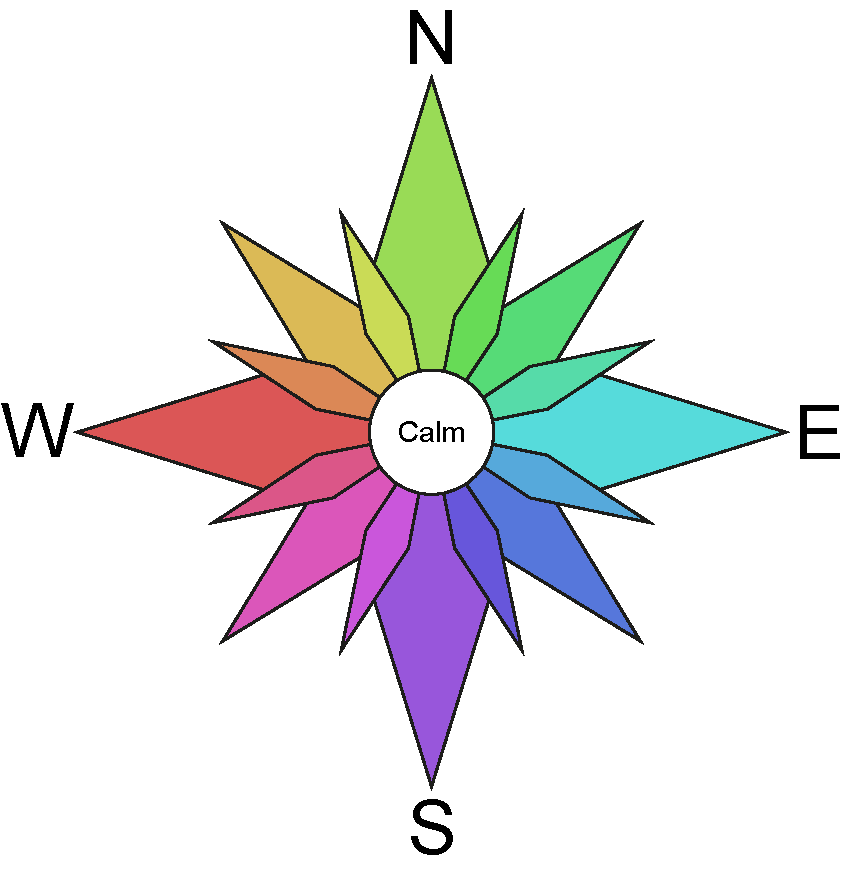
\includegraphics[width=0.3\linewidth]{compass-rose.pdf}
    \caption[Compass Rose mapping colour to wind direction]{
        The mapping of hue to wind direction used for
        \cref{fig:galiwinku-observations,fig:milingimbi-observations,%
        fig:galiwinku-wind-vectors}.  These colours are equidistant in
        the HSL colour space, with constant saturation and lightness.}
    \label{fig:compass-rose}
\end{SCfigure}

\begin{figure}[p]
    \centering
    \includegraphics[width=\linewidth]{galiwinku/climograph.pdf}
    \caption[Monthly Climograph for Galiwinku]{
        Monthly summary of climate statistics at Galiwinku, showing the per-day
        mean for each month.  Rainfall (vertical bars), maximum temperature
        (solid line), minimum temperature (dashed line), and  dewpoint
        temperature (dotted line).  Dewpoint temperature is a measure of humidity.}
    \label{fig:galiwinku-climograph}
\vspace{1cm}
    \centering
    \includegraphics[width=\linewidth]{galiwinku/wind-vectors.pdf}
    \caption[Monthly wind vector summary for Galiwinku]{
        Prevailing wind direction by month and time of day.  Each set of
        lines shows the proportion of wind coming from the corresponding
        point of the compass, with colours given by \cref{fig:compass-rose}.
        Note that each set of lines is scaled to the longest \textit{in
        that set}; this trades comparability for clear visualisation --
        sets with few lines had just as much wind, but from fewer directions.
        }
    \label{fig:galiwinku-wind-vectors}
\end{figure}


The mapping of hue to wind direction shown in \Cref{fig:compass-rose} is
used for \cref{fig:galiwinku-observations,fig:milingimbi-observations,%
fig:galiwinku-wind-vectors}.  These colours are equidistant in the HSL colour space,
which uses a polar (cylindrical) coordinate system for hue, saturation,
and lightness (hence, ``HSL'').  With constant saturation and lightness,
hue can be mapped directly to wind direction and equidistant colours
have similar perceptual difference - at least within reproduction tolerances.
%
The direction-colour mapping was `rotated' - from red at north to red at west -
to ensure that the contrast of prevailing monsoon winds is blue/yellow,
rather than red/green which would disadvantage colourblind readers.

Weather observations at Galiwinku and Milingimbi are shown in
\cref{fig:galiwinku-observations,fig:milingimbi-observations} as a set of
heatmaps (panels, arranged vertically).  \Cref{fig:how-read-multipanel}
gives a detailed walkthrough of how to read these figures.
%
Unlike the climograph above, these figures clearly show variation in timing
of seasonal onset between years.  This demonstrates that timeseries data
at daily resolution are required for investigation of Indigenous seasons.
%
The degree of seasonal variation in each indicator is also clearly visible:
minimum temperature varies more than maximum; wind direction varies more in
the morning while wind speed varies more in the afternoon (both due to the
sea breeze).


% %%%%%%%%%%%%%%%%%%%%%%%%%%%%%%%%%%%%%%%%%%%%%%%%%%%%%%%%%%%%%%%%%%%
% This section gets a little tricky.  We want the multipanels on
% facing pages, and the explainer box immediately before or after.
%
% However, the page(s) aren't filled until after the floats are placed.
% We therefore use \clearpage to get to the top of the first of three
% float pages.  Iff it's odd, don't place the multipanels.  Place the
% explain box.  Iff it's odd, place the multipanels.  This looks
% weird, but works because all conditions check the same page!
% %%%%%%%%%%%%%%%%%%%%%%%%%%%%%%%%%%%%%%%%%%%%%%%%%%%%%%%%%%%%%%%%%%%

\clearpage

\newcommand{\ObservationMultipanels}{
\begin{figure}[p]
    \centering
    \includegraphics[width=\textwidth]{galiwinku/observations.pdf}
    \caption[Historical weather observations at Galiwinku]{
        Weather observations at Galiwinku.  Each panel shows a single variable,
        with years on the y axis and day-of-year on the x.  Note that variables
        have distinct seasonal patterns, the details of which vary each year.
        \Cref{fig:how-read-multipanel} explains how to read this figure.}
    \label{fig:galiwinku-observations}
\end{figure}
\begin{figure}[p]
    \centering
    \includegraphics[width=\textwidth]{milingimbi/observations.pdf}
    \caption[Historical weather observations at Milingimbi Airport]{
        Weather observations at Milingimbi Airport.  Each panel shows a single variable,
        with years on the y axis and day-of-year on the x.  Note that variables
        have distinct seasonal patterns, the details of which vary each year.
        \Cref{fig:how-read-multipanel} explains how to read this figure.}
    \label{fig:milingimbi-observations}
\end{figure}
}

\checkoddpage\ifoddpage\ObservationMultipanels\fi

\begin{framedbox}
\caption[How to read multipanel heatmaps]{How to read multipanel heatmaps}
\label{fig:how-read-multipanel}
    \setlength{\parskip}{4pt}           % per preamble for whole document
    \setlength{\parindent}{17.62482pt}  % default value, per \the\parindent

    Multipanel heatmaps have several advantages: they concisely express a
    great deal of data, and make trends or variability between years clearly
    visible.  They are designed to show all the details of heterogenous data
    that would usually be hidden by sumarising or aggregating it to a simpler
    form.  Detail sometimes comes at the expense of readability, so this tutorial
    walks through how to read and interpret \cref{fig:galiwinku-observations},
    which shows forty-eight thousand weather observations taken at Galiwinku.

    Each heatmap is a grid, with year on the y-axis and day-of-year on the
    x-axis.  Each cell is then shaded according
    to the value observed on that day; days  without data are shaded black.
    Years of observation are printed to the left of each panel, as y-axis labels.
    At the bottom of the figure, the x-axis is labelled by month -- the data
    are daily, but numerical day-of-year labels are generally unintuitive.
    To the left of each panel is the colour key, and the name of the variable.
    This color key is identical for panels of the same variable across all
    figures, for easier comparison.

    The topmost panel shows the five-day mean for daily rainfall.
    The first row of data is mostly black, indicating missing
    values -- this station began observations in October 1999.  Other gaps,
    where the record was interrupted for a few days or weeks, are visible in
    all panels; apparently the station was mostly non-functional between June
    and October 2015.
    %
    Rainfall is clearly seasonal, but also intermittent:  there are a series
    of large rainfall events in most years until late-April, then little if any
    rainfall until November.

    The next panels show maximum and minimum temperature.  Note the scale to
    the right of the panel - even the lowest minimum temperatures rarely drop
    below 18 $^\circ$C.  Daily maximum temperature fluctuates in the
    early months of the year, and careful inspection hints that relatively
    low temperatures may be related to heavy rainfall.

    The bottom four panels are probably the most complex, and form two pairs:
    wind speed and direction in the morning (9am), and in the afternoon (3pm).
    %
    The blue shaded panels show wind speed.  Until March, wind speed at
    both times is dominated by rainfall events -- knowing that the wind is also
    high, we could properly call them storms -- and in later months a clear
    divergence is visible, showing that the sea breeze is most notable from
    September onwards.
    %
    The multi-coloured panels show wind direction; \cref{fig:compass-rose} gives
    the key.  The morning data show a clear westerly / south-easterly / northerly
    wind regime through the year, while the afternoon wind -- sea breeze --
    tends to blow mainly from the north or (less often) south-east.
    (for an explanation, see the discussion of these results)
\end{framedbox}

\checkoddpage\ifoddpage\else\ObservationMultipanels\fi


\section{Quantifying a Yolngu Calendar}
\label{sec:applying-seasons-method}

In this section, the qualitative data describing a Yolngu seasonal
calendar is applied to the observational weather record, deriving
a numerical specification for each season and ultimately a best-effort
timeseries of which season was `observed' on each day.
%
For readability, only figures for the seasons at Galiwinku
(Ngayawili weather station) are included in the text.  Corresponding
figures for all other stations can be found in the electronic appendices.


\begin{table}[h]
    \centering
    \caption{A quantifiable summary of the Yolngu seasons case study.}
    \label{tab:quant-seasons-summary}
    \sffamily\small
    \begin{tabular}{llllll}
        Season          &  Typical Months       &  Criteria to recognise                    \\
        \noalign{\vskip 0.5em}\hline\noalign{\vskip 0.5em}
        Dhuludur        &  Oct, Nov, Dec        &  Cool at night, mixed wind, first rain    \\
        Barramirri      &  Dec, Jan, Feb        &  NW wind, heavy rain most days            \\
        Mayaltha        &  Feb, Mar             &  NW wind, approx weekly rain              \\
        Midawarr        &  Mar, Apr, May        &  NE to E wind, less rain, last storm      \\
        Dharrathamirri  &  May, Jun, Jul, Aug   &  No rain, consistent ESE-SSE wind         \\
        Rarrandharr     &  Sep, Oct             &  Hot days, low humidity
    \end{tabular}
\end{table}

Typical timing and recognition criteria for each season are summarised in
\cref{tab:quant-seasons-summary}.  Python3 code implementing these criteria
is listed in \cref{fig:season-definitions-code}; the blue-shaded panels in
\cref{fig:galiwinku-seasons} display normalised output from application of
this code to the weather record.

\begin{framedbox}
    \lstinputlisting[firstline=36, lastline=63, xleftmargin=0.1\textwidth]{../code/season.py}
    \centering
    \caption[Python code: definition of season indices]{
        Code listing of variables and conditions used to detect seasons.
        Seasons are defined by numerical criteria for each day, such as
        ``rainfall greater than 15mm'', or ``maximum temperature below mean''.
        Applying a criterion to the weather data gives a timeseries with 1 or 0
        for each day, and the raw index for each season is the element-wise
        sum of these timeseries.}
    \label{fig:season-definitions-code}
\end{framedbox}


\begin{SCfigure}[][h]
    \centering
    \includegraphics[width=0.7\textwidth]{galiwinku/season-pie.pdf}
    \caption[Calculated season frequency, Galiwinku]{
        Proportion of days on which each season was observed at
        Galiwinku, over the period of available data.
        These colours are used for each season in all figures below.
        Note that this figure shows proportional duration, but does
        not represent onset timing; seasons do not always occur over
        contiguous periods.
        }
    \label{fig:galiwinku-season-pie}
\end{SCfigure}


The figures in this section fall into two distinct but related categories.
Understanding this distinction and the relationship between them is crucial
for accurate interpretation -- both attempt to summarise the data shown in
\cref{fig:galiwinku-seasons} (parts of which fall into each category) without
erasing or misrepresenting the variability that is a key characteristic of
Yolngu seasons.


\Cref{fig:galiwinku-seasons} is a multi-panel heatmap, using the same format
as \cref{fig:galiwinku-observations,fig:milingimbi-observations} above.
Each season has an individual panel showing the index for that season on each
day, derived by taking the raw index from \cref{fig:season-definitions-code}
and applying a four-day rolling mean and converting to a z-score (standard
deviations from the mean) to allow direct comparison between indices.
%
The topmost panel is an aggregated version, showing which season on each day
had the greatest index -- the crucial timeseries for any further analysis.

Note the clear distinction between Midawarr (purple), Dharrathamirri (yellow),
and Rarrandharr (light blue) -- the dry seasons.  This clear pattern in the
all-seasons panel arises from the distinctive and largely non-overlapping
peaks in the index value for each season, forming a diagonal pattern over
the lower three panels.
%
On the other hand, Dhuludur (dark blue), Barramirri (green), and Mayaltha
(red) are not clearly distinguished in their individual patterns.  This
manifests in mixed occurance shown on the all-seasons panel, and is also
clearly visible in the summarising figures below.


\begin{figure}[p]
    \centering
    \includegraphics[width=\textwidth]{galiwinku/seasons.pdf}
    \caption[Detected seasons for Galiwinku]{
        Detected seasons at Galiwinku, based on threshold conditions
        shown in \cref{fig:season-definitions-code}.

        This figure shows the normalised index for each season --
        the mean and sum of each panel is zero.  Higher values
        (darker) indicate a better match between weather
        conditions on that day and the description of that season.
        }
    \label{fig:galiwinku-seasons}
\end{figure}


The first category is those figures showing a \textit{normalised index of
seasonal intensity} -- the z-score of the indices calculated in
\cref{fig:season-definitions-code}.  These indices can be thought of as scoring
how well conditions on some day match the definition of each season.
The full data is shown by the blue-shaded panels in \cref{fig:galiwinku-seasons},
and the mean (aggregated by day-of-year) is shown in \cref{fig:season-daily-index}.

The second category shows a further step of processing, where each day in
the dataset is assigned to the season with the greatest index on that day.
These figures all share the colour scheme used by \cref{fig:galiwinku-season-pie},
which simply shows the proportion of days assigned to each season.
The full data is shown by the top-most panel in \cref{fig:galiwinku-seasons},
and shown in aggregate (proportion of days for each day-of-year) in
\Cref{fig:season-daily-prob}.  The proportional area of each season (colour)
is equal across these figures, as they represent the same data in more
or less abstracted formats.

The degree of distinction between seasons is shown as a line chart in
\cref{fig:season-daily-index}, showing the mean per-day index for each
season.  This shows ; lines of similar heights show seasons which describe
typical conditions with similar predictive power.  That Dharrathamirri
has the highest peak means it is most distinct -- southeast wind and no
rain describes it well, and also matches other seasons very poorly.
Note however that these indices are independent.

A different approach is demonstrated in \cref{fig:season-daily-prob}, showing
empirical probability of observing each season on a given day of the year.
These data are further smoothed by a running weekly mean, to remove noise
introduced by the small sample size (only 10-15 years for each station).

This tells a similar story to the index lines, but readers should note
that these figures are seperately derived from the data shown in
\cref{fig:galiwinku-seasons}.  Most importantly, observed occurance
rates are not independent -- when one season is observed more, others
must be observed proportionally less.  This property amplifies the
difference between indices on a year-by-year basis, which clearly
shows variability between years or `strong second' finishes.


\begin{figure}[p]
    \centering
    \includegraphics[width=\textwidth]{galiwinku/seasons-daily-index.pdf}
    \caption[Season index by day-of-year, Elcho Island]{
        Mean normalised (z-score) index for seasons per day-of-year
        at Galiwinku.  Note the clear distinction in the dry season,
        but muddle in the Wet (Dec-Feb).
        This is not indicative of poor detection on a single day,
        but rather that occurence varies more between years.
        }
    \label{fig:season-daily-index}
\vspace{1cm}
    \includegraphics[width=\textwidth]{galiwinku/seasons-daily-prob.pdf}
    \caption[Season probability by day-of-year, Elcho Island]{
        Observed probability of each season by day of year.
        This figure does not show consistently strong ordering among all
        seasons; this may be attributed to a combination of imperfect
        detection, true variation in seasonal occurance, and details
        lost in aggregation.
        }
    \label{fig:season-daily-prob}
\end{figure}


Monthly means for the normalised index of each season and most common season
in each month are shown in \cref{tab:galiwinku-monthly-summary}.  This is
a simplified textual form of \cref{fig:season-daily-prob,fig:season-daily-index}.


\begin{table}[h]
    \caption[Most common season and indices by month]{
        Most common season at Galiwinku by month, and monthly mean season
        indices.  `Main Season' summarises the data shown in
        \cref{fig:season-daily-prob}, while the per-season index columns
        are equivalent to \cref{fig:season-daily-index}.
        }
    \label{tab:galiwinku-monthly-summary}
    \sffamily\small\centerline{
    \begin{tabular}{llrrrrrr}
        Month & Main Season &  Dhuludur &  Barramirri & %
        Mayaltha &  Midawarr &  Dharrathamirri &  Rarrandharr \\
        \noalign{\vskip 0.5em}\hline\noalign{\vskip 0.5em}
        Jan &      Barramirri &   0.8 &   1.2 &   0.9 &  -0.4 &  -1.1 &  -0.9  \\
        Feb &      Barramirri &   0.6 &   1.1 &   0.8 &  -0.4 &  -1.0 &  -1.0  \\
        Mar &        Midawarr &   0.3 &   0.5 &   0.2 &   0.1 &  -0.8 &  -0.9  \\
        Apr &        Midawarr &  -0.6 &  -0.5 &  -0.5 &   1.0 &   0.0 &  -0.3  \\
        May &  Dharrathamirri &  -1.0 &  -0.9 &  -0.5 &   0.5 &   0.9 &   0.1  \\
        Jun &  Dharrathamirri &  -0.9 &  -0.9 &  -0.5 &  -0.5 &   1.3 &   0.2  \\
        Jul &  Dharrathamirri &  -0.8 &  -0.9 &  -0.5 &  -0.1 &   1.3 &   0.2  \\
        Aug &  Dharrathamirri &  -0.5 &  -0.8 &  -0.5 &   0.2 &   1.0 &   0.5  \\
        Sep &     Rarrandharr &   0.1 &  -0.5 &  -0.4 &   0.3 &   0.3 &   1.0  \\
        Oct &     Rarrandharr &   0.5 &  -0.0 &  -0.1 &   0.0 &  -0.2 &   0.9  \\
        Nov &     Rarrandharr &   0.6 &   0.5 &   0.3 &  -0.3 &  -0.6 &   0.4  \\
        Dec &        Mayaltha &   0.7 &   0.9 &   0.5 &  -0.3 &  -0.9 &  -0.3  \\
    \end{tabular}
    }
\end{table}



\section{Correlations with Climatic indices}
\label{sec:indices-correlations}

\todo{Add intro/flags to start of section for better flow}
\todo{analyse correlations between seasons and ENSO index/indices, IOD, etc.}


